\section{案例研究:线性生成器}

在这一节中,我们将看到两个由线性函数构建的 PRG 的例子。这两个生成器都遵循 \ref{subsec:3-4-2} 小节中介绍的 Blum-Micali 范式。我们的第一个例子称为\emph{线性同构生成器},它是完全不安全的。我们之所以以它为例,是想举例说明攻击 PRG 时可能会出现的一些优美的数学构造。我们的第二个例子称为\emph{子集和生成器},如果我们假设经典子集和问题的某个特定版本是困难的,就可以证明它是一个安全的 PRG。

\subsection{一个密码分析的例子:线性同构生成器}

线性同构生成器(linear congruential generators, LCG) 常被用来在统计模拟中产生伪随机值。它们速度快,易实现,并且被广泛部署。LCG 的几个变体也被用于早期的 glibc、Microsoft Visual Basic 和 Java 运行时中,目的是为了提供随机元。尽管这些生成器用于模拟是足够的,但它们\emph{绝不}应该用在密码学应用中,因为它们作为 PRG 是不安全的。尤其是,它们是可预测的:给定 LCG 的连续若干输出,我们很容易计算出所有后续的输出。在本节中,我们通过展示一种预测算法来描述针对 LCG 的攻击。

基本的线性同构生成器由四个公共系统参数指定:一个整数 $q$,两个常数 $a,b\in\{0,\dots,q-1\}$,以及一个正整数 $w\leq q$。选取的常数 $a$ 应与 $q$ 互素。我们用 $\mathcal{S}_q$ 和 $\mathcal{R}$ 来表示集合:
\[
\mathcal{S}_q:=\{0,\dots,q-1\},
\quad
\mathcal{R}:=\{0,\dots,\lfloor(q-1)/w\rfloor\}
\]
这里,$\lfloor\cdot\rfloor$ 表示向下取整:对于一个实数 $x$,$\lfloor x\rfloor$ 是小于或等于 $x$ 的最大整数。现在,以$s\in\mathcal{S}_q$ 为种子的生成器 $G_\mathrm{lcg}:\mathcal{S}_q\to\mathcal{R}\times\mathcal{S}_q$ 的定义如下:
\[
G_\mathrm{lcg}(s)
:=
\big(
\lfloor s/w \rfloor,\;
as+b\bmod q
\big)
\]
当 $w$ 是 $2$ 的整数次幂,比如 $w=2^t$ 时,$\lfloor s/w \rfloor$ 其实就是简单地抹除 $s$ 的 $t$ 个最小有效比特。因此,$G_\mathrm{lcg}(s)$ 的表达式的前半部分就是抹去 $s$ 的 $t$ 个最小有效比特后的结果。

生成器 $G_\mathrm{lcg}(s)$ 显然是不安全的,因为只要给定 $s':=as+b\bmod q$,我们就可以直接重建 $s$,然后将 $\lfloor s/w \rfloor$ 从随机值中区分出来。然而,考虑下面的一种 Blum-Micali 构造的变体,其中,最终的 $\mathcal{S}_q$ 中的值不会被输出:

\vspace*{10pt}

\hspace*{5pt} $G_\mathrm{lcg}^{(n)}(s):=$
\hspace*{20pt} $s_0\leftarrow s$\\
\hspace*{100pt} 对于 $i\leftarrow 1$ 到 $n$:\\
\hspace*{100pt} \quad\quad\quad
$r_i\leftarrow\lfloor s_{i-1}/w \rfloor$,
\quad
$s_i\leftarrow as_{i-1}+b\bmod q$\\
\hspace*{100pt} 输出 $(r_0,\dots,r_n)$。

\vspace*{10pt}

\noindent
我们将每一次循环称为 LCG 的一次迭代,并称 $r_1,\dots,r_n$ 中的元素为一次迭代的输出。

不同的实现会使用不同的系统参数 $q$,$a$,$b$ 和 $w$。例如,Java 8 中的 \texttt{Math.random} 函数使用的是 $q=2^{48}$,$w=2^{22}$ 以及十六进制常数 $a=\texttt{0x5DEECE66D}$,$b=\texttt{0x0B}$。因此,LCG 的每次迭代都会输出 $48$ 比特状态 $s_i$ 的前 $48-22=26$ 比特。

这个 Java 8 生成器所使用的参数对于安全应用来说显然太小了,因为生成器的第一次迭代输出就会揭示 $s$ 中除了 $22$ 比特之外的所有其他比特。攻击者可以通过穷举搜索轻易地恢复未知的这 $22$ 比特:对于这 $22$ 比特的每一个可能值,它都生成一个候选种子 $\hat s$。它可以从 $\hat s$ 出发计算若干个后续输出,并将其与从实际的生成器中观察到的后续比特进行对比,以此来测试 $\hat s$ 是否是正确的种子。只要遍历所有 $2^{22}$ 个候选种子(约 $400$ 万个),攻击者就能最终找到正确的种子 $s$,然后就可以预测生成器的所有后续输出。这种攻击在现代处理器上的运行时间甚至不会超过一秒。

就算 LCG 的参数大到足以抵抗穷举搜索,比如说令 $q=2^{512}$,生成器 $G_\mathrm{lcg}^{(n)}$ 也是不安全的。就算你可以从各种软件库中找到它,也永远不要把它用在安全应用中。已知的针对 LCG 的攻击表明,即使生成器每次迭代只输出几个比特,我们仍有可能基于几个连续的输出预测整个序列。让我们看看一种优雅的攻击方式。

\begin{snote}[密码分析。]
假设 $q$ 很大(例如 $q=2^{512}$),LCG $G_\mathrm{lcg}^{(n)}$ 的每次迭代都会输出状态 $s$ 中大约一半的比特,就像 Java 8 中的 \texttt{Math.random} 生成器那样。考虑到种子 $s$ 的大小,对其进行穷举搜索是不可能的。然而,我们下面将会展示,如何用仅仅两次连续迭代的输出来快速地预测生成器。

更确切地说,假设对于某个固定的 $c>0$,例如 $c=32$,我们有 $w<\sqrt{q}/c$。这就意味着在每次迭代中,生成器所输出的比特数都只略多于当前内部状态的比特数的一半。

假设攻击者得到了生成器的连续两个输出 $r_i,r_{i+1}\in\mathcal{R}$。我们下面展示它预测剩余序列的方法。对于某个未知的 $s_i\in\mathcal{S}_q$,攻击者知道:
\[
r_i=\lfloor s_i/w\rfloor,
\quad\quad
r_{i+1}=\lfloor s_{i+1}/w\rfloor=\lfloor(as_i+b\bmod q)/w\rfloor
\]
我们有:
\[
r_i\cdot w+e_0=s_i,\quad\quad
r_{i+1}\cdot w+e_1=(as_i+b\bmod q)
\]
其中,$e_0$ 和 $e_1$ 是 $s_i$ 和 $s_{i+1}$ 除以 $w$ 后的余数;特别地,我们有 $0\leq e_0$,且 $e_1<w<\sqrt{q}/c$。$e_0$ 和 $e_1$ 都小于 $\sqrt{q}$ 这一事实是攻击能够成功的一个重要因素。接下来,我们用 $s$ 代换 $s_i$,并引入一个整数变量 $x$ 来消除 $\mathrm{mod}\;q$,得到:
\[
r_i\cdot w+e_0=s,\quad\quad
r_{i+1}\cdot w+e_1=as+b+qx
\]
$x$,$s$,$e_0$ 和 $e_1$ 对于攻击者来说都是未知的,但它知道 $r_i$,$r_{i+1}$,$w$,$a$ 和 $b$。最后,重新排列各项,把涉及 $x$ 和 $s$ 的项都放到左边,得到:
\begin{equation}\label{eq:3-12}
s=r_i\cdot w+e_0,
\quad\quad
as+qx=r_{i+1}w-b+e_1
\end{equation}
我们可以将式 \ref{eq:3-12} 重写为向量形式:
\begin{equation}
s\cdot
\begin{pmatrix}
1\\a
\end{pmatrix}
+x\cdot
\begin{pmatrix}
0\\q
\end{pmatrix}
=\boldsymbol{g}+\boldsymbol{e}
\quad\quad
\text{其中}
\quad\quad
\boldsymbol{g}:=
\begin{pmatrix}
r_iw\\r_{i+1}w-b
\end{pmatrix}
,\;\;
\boldsymbol{e}:=
\begin{pmatrix}
e_0\\e_1
\end{pmatrix}
\end{equation}
令 $\boldsymbol{u}\in\mathbb{Z}^2$ 表示未知向量 $\boldsymbol{u}:=\boldsymbol{g}+\boldsymbol{e}=s\cdot(1,a)^\mathrm{T}+x\cdot(0,q)^\mathrm{T}$。如果攻击者能够找到 $\boldsymbol{u}$,它就可以通过线性代数计算轻松地从 $\boldsymbol{u}$ 中恢复 $s$ 和 $x$。利用 $s$,它就可以预测 PRG 的其余输出。因此,想要破解生成器,只需要找到这样的向量 $\boldsymbol{u}$ 即可。攻击者知道向量 $\boldsymbol{g}\in\mathbb{Z}^2$,此外,它也知道 $\boldsymbol{e}$ 是很短的,即 $\lVert\boldsymbol{e}\rVert_\infty$ 最大为 $\sqrt{q}/c$。因此,它知道 $\boldsymbol{u}$ 是``接近" $\boldsymbol{g}$ 的。

我们下面展示如何由 $\boldsymbol{g}$ 找到 $\boldsymbol{u}$。考虑向量 $(1,a)^\mathrm{T}$ 和 $(0,q)^\mathrm{T}$ 的所有整系数线性组合所构成的集合。我们用 $\mathcal{L}_a$ 表示这个集合,它是 $\mathbb{Z}^2$ 的一个子集,包含像 $(1,a)^\mathrm{T}$,$(2,2a)^\mathrm{T}$ 和 $(3,3a-2q)^\mathrm{T}$ 这样的向量。图 \ref{fig:3-9} 展示了集合 $\mathcal{L}_a$,图中的实心点都是向量 $(1,a)^\mathrm{T}$ 和 $(0,q)^\mathrm{T}$ 的整系数线性组合。我们称集合 $\mathcal{L}_a$ 是由向量 $(1,a)^\mathrm{T}$ 和 $(0,q)^\mathrm{T}$ 生成的二维\textbf{网格(lattice)}。

\begin{figure}
	\centering
	\tikzset{every picture/.style={line width=0.75pt}}

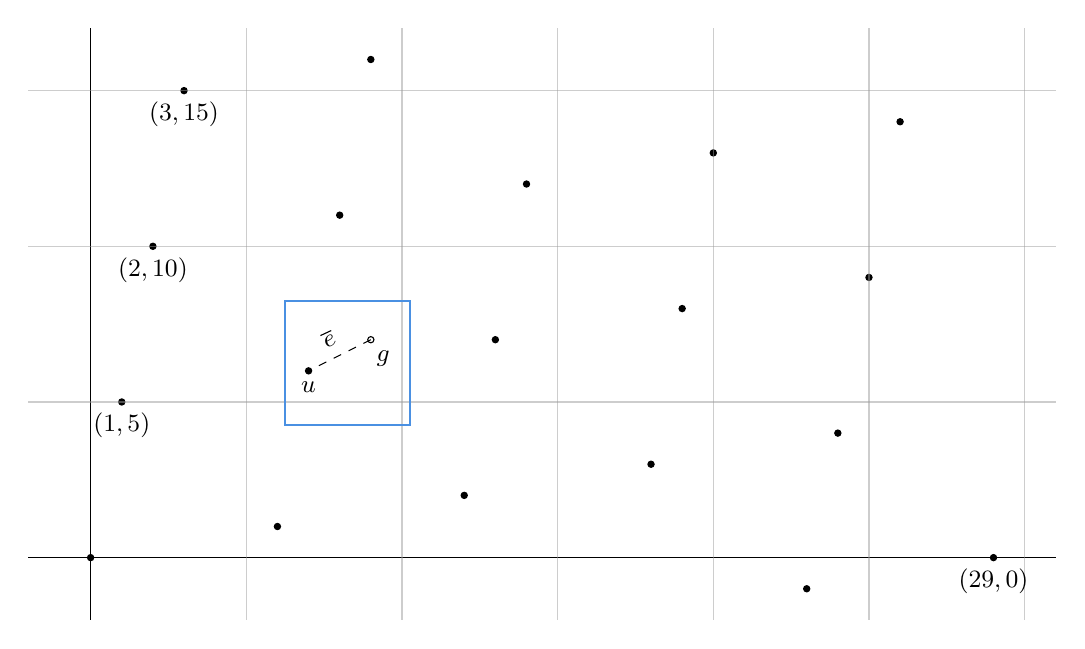
\begin{tikzpicture}[x=0.75pt,y=0.75pt,yscale=-0.75,xscale=0.75]

\draw    (40,0) -- (40,380) ;
\draw    (0,340) -- (660,340) ;

\draw  [fill={rgb, 255:red, 0; green, 0; blue, 0 }  ,fill opacity=1 ] (98,40) .. controls (98,38.9) and (98.9,38) .. (100,38) .. controls (101.1,38) and (102,38.9) .. (102,40) .. controls (102,41.1) and (101.1,42) .. (100,42) .. controls (98.9,42) and (98,41.1) .. (98,40) -- cycle ;
\draw  [fill={rgb, 255:red, 0; green, 0; blue, 0 }  ,fill opacity=1 ] (38,340) .. controls (38,338.9) and (38.9,338) .. (40,338) .. controls (41.1,338) and (42,338.9) .. (42,340) .. controls (42,341.1) and (41.1,342) .. (40,342) .. controls (38.9,342) and (38,341.1) .. (38,340) -- cycle ;
\draw  [fill={rgb, 255:red, 0; green, 0; blue, 0 }  ,fill opacity=1 ] (58,240) .. controls (58,238.9) and (58.9,238) .. (60,238) .. controls (61.1,238) and (62,238.9) .. (62,240) .. controls (62,241.1) and (61.1,242) .. (60,242) .. controls (58.9,242) and (58,241.1) .. (58,240) -- cycle ;
\draw  [fill={rgb, 255:red, 0; green, 0; blue, 0 }  ,fill opacity=1 ] (78,140) .. controls (78,138.9) and (78.9,138) .. (80,138) .. controls (81.1,138) and (82,138.9) .. (82,140) .. controls (82,141.1) and (81.1,142) .. (80,142) .. controls (78.9,142) and (78,141.1) .. (78,140) -- cycle ;
\draw  [fill={rgb, 255:red, 0; green, 0; blue, 0 }  ,fill opacity=1 ] (178,220) .. controls (178,218.9) and (178.9,218) .. (180,218) .. controls (181.1,218) and (182,218.9) .. (182,220) .. controls (182,221.1) and (181.1,222) .. (180,222) .. controls (178.9,222) and (178,221.1) .. (178,220) -- cycle ;
\draw  [fill={rgb, 255:red, 0; green, 0; blue, 0 }  ,fill opacity=1 ] (438,80) .. controls (438,78.9) and (438.9,78) .. (440,78) .. controls (441.1,78) and (442,78.9) .. (442,80) .. controls (442,81.1) and (441.1,82) .. (440,82) .. controls (438.9,82) and (438,81.1) .. (438,80) -- cycle ;
\draw  [fill={rgb, 255:red, 0; green, 0; blue, 0 }  ,fill opacity=1 ] (278,300) .. controls (278,298.9) and (278.9,298) .. (280,298) .. controls (281.1,298) and (282,298.9) .. (282,300) .. controls (282,301.1) and (281.1,302) .. (280,302) .. controls (278.9,302) and (278,301.1) .. (278,300) -- cycle ;
\draw  [fill={rgb, 255:red, 0; green, 0; blue, 0 }  ,fill opacity=1 ] (218,20) .. controls (218,18.9) and (218.9,18) .. (220,18) .. controls (221.1,18) and (222,18.9) .. (222,20) .. controls (222,21.1) and (221.1,22) .. (220,22) .. controls (218.9,22) and (218,21.1) .. (218,20) -- cycle ;
\draw  [fill={rgb, 255:red, 0; green, 0; blue, 0 }  ,fill opacity=1 ] (558,60) .. controls (558,58.9) and (558.9,58) .. (560,58) .. controls (561.1,58) and (562,58.9) .. (562,60) .. controls (562,61.1) and (561.1,62) .. (560,62) .. controls (558.9,62) and (558,61.1) .. (558,60) -- cycle ;
\draw  [fill={rgb, 255:red, 0; green, 0; blue, 0 }  ,fill opacity=1 ] (198,120) .. controls (198,118.9) and (198.9,118) .. (200,118) .. controls (201.1,118) and (202,118.9) .. (202,120) .. controls (202,121.1) and (201.1,122) .. (200,122) .. controls (198.9,122) and (198,121.1) .. (198,120) -- cycle ;
\draw  [fill={rgb, 255:red, 0; green, 0; blue, 0 }  ,fill opacity=1 ] (318,100) .. controls (318,98.9) and (318.9,98) .. (320,98) .. controls (321.1,98) and (322,98.9) .. (322,100) .. controls (322,101.1) and (321.1,102) .. (320,102) .. controls (318.9,102) and (318,101.1) .. (318,100) -- cycle ;
\draw  [fill={rgb, 255:red, 0; green, 0; blue, 0 }  ,fill opacity=1 ] (498,360) .. controls (498,358.9) and (498.9,358) .. (500,358) .. controls (501.1,358) and (502,358.9) .. (502,360) .. controls (502,361.1) and (501.1,362) .. (500,362) .. controls (498.9,362) and (498,361.1) .. (498,360) -- cycle ;
\draw  [fill={rgb, 255:red, 0; green, 0; blue, 0 }  ,fill opacity=1 ] (158,320) .. controls (158,318.9) and (158.9,318) .. (160,318) .. controls (161.1,318) and (162,318.9) .. (162,320) .. controls (162,321.1) and (161.1,322) .. (160,322) .. controls (158.9,322) and (158,321.1) .. (158,320) -- cycle ;
\draw  [fill={rgb, 255:red, 0; green, 0; blue, 0 }  ,fill opacity=1 ] (518,260) .. controls (518,258.9) and (518.9,258) .. (520,258) .. controls (521.1,258) and (522,258.9) .. (522,260) .. controls (522,261.1) and (521.1,262) .. (520,262) .. controls (518.9,262) and (518,261.1) .. (518,260) -- cycle ;
\draw  [fill={rgb, 255:red, 0; green, 0; blue, 0 }  ,fill opacity=1 ] (618,340) .. controls (618,338.9) and (618.9,338) .. (620,338) .. controls (621.1,338) and (622,338.9) .. (622,340) .. controls (622,341.1) and (621.1,342) .. (620,342) .. controls (618.9,342) and (618,341.1) .. (618,340) -- cycle ;
\draw  [fill={rgb, 255:red, 255; green, 255; blue, 255 }  ,fill opacity=1 ] (218,200) .. controls (218,198.9) and (218.9,198) .. (220,198) .. controls (221.1,198) and (222,198.9) .. (222,200) .. controls (222,201.1) and (221.1,202) .. (220,202) .. controls (218.9,202) and (218,201.1) .. (218,200) -- cycle ;
\draw  [fill={rgb, 255:red, 0; green, 0; blue, 0 }  ,fill opacity=1 ] (398,280) .. controls (398,278.9) and (398.9,278) .. (400,278) .. controls (401.1,278) and (402,278.9) .. (402,280) .. controls (402,281.1) and (401.1,282) .. (400,282) .. controls (398.9,282) and (398,281.1) .. (398,280) -- cycle ;
\draw  [fill={rgb, 255:red, 0; green, 0; blue, 0 }  ,fill opacity=1 ] (298,200) .. controls (298,198.9) and (298.9,198) .. (300,198) .. controls (301.1,198) and (302,198.9) .. (302,200) .. controls (302,201.1) and (301.1,202) .. (300,202) .. controls (298.9,202) and (298,201.1) .. (298,200) -- cycle ;
\draw  [fill={rgb, 255:red, 0; green, 0; blue, 0 }  ,fill opacity=1 ] (418,180) .. controls (418,178.9) and (418.9,178) .. (420,178) .. controls (421.1,178) and (422,178.9) .. (422,180) .. controls (422,181.1) and (421.1,182) .. (420,182) .. controls (418.9,182) and (418,181.1) .. (418,180) -- cycle ;
\draw  [fill={rgb, 255:red, 0; green, 0; blue, 0 }  ,fill opacity=1 ] (538,160) .. controls (538,158.9) and (538.9,158) .. (540,158) .. controls (541.1,158) and (542,158.9) .. (542,160) .. controls (542,161.1) and (541.1,162) .. (540,162) .. controls (538.9,162) and (538,161.1) .. (538,160) -- cycle ;


\draw [color={rgb, 255:red, 155; green, 155; blue, 155 }  ,draw opacity=0.5 ][line width=0.5] (140,0) -- (140,380) ;
\draw [color={rgb, 255:red, 155; green, 155; blue, 155 }  ,draw opacity=0.5 ][line width=0.5]   (240,0) -- (240,380) ;
\draw [color={rgb, 255:red, 155; green, 155; blue, 155 }  ,draw opacity=0.5 ][line width=0.5]   (340,0) -- (340,380) ;
\draw [color={rgb, 255:red, 155; green, 155; blue, 155 }  ,draw opacity=0.5 ][line width=0.5]   (440,0) -- (440,380) ;
\draw [color={rgb, 255:red, 155; green, 155; blue, 155 }  ,draw opacity=0.5 ][line width=0.5]   (540,0) -- (540,380) ;
\draw [color={rgb, 255:red, 155; green, 155; blue, 155 }  ,draw opacity=0.5 ][line width=0.5]   (640,0) -- (640,380) ;

\draw [color={rgb, 255:red, 155; green, 155; blue, 155 }  ,draw opacity=0.5 ][line width=0.5]   (0,240) -- (660,240) ;
\draw [color={rgb, 255:red, 155; green, 155; blue, 155 }  ,draw opacity=0.5 ][line width=0.5]   (0,140) -- (660,140) ;
\draw [color={rgb, 255:red, 155; green, 155; blue, 155 }  ,draw opacity=0.5 ][line width=0.5]   (0,40) -- (660,40) ;

\draw  [dash pattern={on 3pt off 3pt}]  (220,200) -- (180,220) ;
\draw  [color={rgb, 255:red, 74; green, 144; blue, 226 }  ,draw opacity=1][line width=0.8]  (165,175) -- (245,175) -- (245,255) -- (165,255) -- cycle ;


\draw (100,45.4) node [anchor=north] [inner sep=0.75pt]  [font=\small]  {$( 3,15)$};
\draw (80,145.4) node [anchor=north] [inner sep=0.75pt]  [font=\small]  {$( 2,10)$};
\draw (60,245.4) node [anchor=north] [inner sep=0.75pt]  [font=\small]  {$( 1,5)$};
\draw (620,345.4) node [anchor=north] [inner sep=0.75pt]  [font=\small]  {$( 29,0)$};
\draw (180,225.4) node [anchor=north] [inner sep=0.75pt]  [font=\small]  {${\boldsymbol u}$};
\draw (222,205.4) node [anchor=north west][inner sep=0.75pt]  [font=\small]  {${\boldsymbol g}$};
\draw (184.94,195.57) node [anchor=north west][inner sep=0.75pt]  [font=\small,rotate=-335]  {$\overline{e}$};


\end{tikzpicture}
	\caption{与攻击LCG相关的二维网格。这里的网格是由向量$(1,5)^\mathrm{T}$和$(0,29)^\mathrm{T}$生成的。攻击者持有向量$\boldsymbol{g}=(9,7)^\mathrm{T}$,并希望找到最接近的网格向量$\boldsymbol{u}$。在这本图中确实只有一个``接近" $\boldsymbol{g}$ 的网格向量。}
	\label{fig:3-9}
\end{figure}

现在,攻击者有一个向量 $\boldsymbol{g}\in\mathbb{Z}^2$,并且知道它的目标向量 $\boldsymbol{u}\in\mathcal{L}_a$ 接近 $\boldsymbol{g}$。如果它能在 $\mathcal{L}_a$ 中找到与 $\boldsymbol{g}$ 最接近的向量,那么这个向量很有可能就是所需的向量 $\boldsymbol{u}$。下面的定理将表明,对于大多数的 $a\in\mathcal{S}_q$ 来说,情况就是如此。
\end{snote}

\begin{lemma}\label{lemma:3-7}
对于 $\mathcal{S}_q$ 上至少 $(1-16/c^2)\cdot q$ 个 $a$,网格 $\mathcal{L}_a\subseteq\mathbb{Z}^2$ 有如下性质:对于每个 $\boldsymbol{g}\in\mathbb{Z}^2$,最多只存在一个向量 $\boldsymbol{u}\in\mathcal{L}_a$ 满足 $\lVert\boldsymbol{g}-\boldsymbol{u}\rVert_\infty < \sqrt{q}/c$。
\end{lemma}

在引理 \ref{lemma:3-7} 中取 $c=32$(则 $w=\sqrt{q}/30$),那么对于 $98\%$ 的 $a\in\mathcal{S}_q$ 来说,$\mathcal{L}_a$ 上离 $\boldsymbol{g}$ 最近的向量恰好就是所需的向量 $\boldsymbol{u}$。在证明该引理之前,我们首先完成对攻击的描述。

剩下的工作就是有效地找到 $\mathcal{L}_a$ 上离 $\boldsymbol{g}$ 最近的向量。这个问题是一个更一般的问题的特例,它叫做\textbf{最近向量问题(closest vector problem)}:给定一个网格 $\mathcal{L}$ 和一个向量 $\boldsymbol{g}$,找到 $\mathcal{L}$ 上离 $\boldsymbol{g}$ 最近的向量。有了这个算法,攻击者就可以根据生成器的两个输出 $r_i$ 和$r_{i+1}$ 恢复 LCG 的内部状态 $s_i$,并预测剩余的序列。这种攻击对 $98\%$ 的 $a\in\mathcal{S}_q$ 都有效。

完整起见,我们注意到,在剩下的 $2\%$ 中,一些 $a\in\mathcal{S}_q$ 所发起的攻击会失败,比如 $a=1$ 和 $a=2$。对于这些 $a$,在 $\mathcal{L}_a$ 上可能会有多个接近给定的 $\boldsymbol{g}$ 的网格向量。我们把设计一个对于 $\mathcal{S}_q$ 上那些不适用于引理 \ref{lemma:3-7} 的 $a$ 有效的攻击作为一个有趣的练习。最后,我们证明引理 \ref{lemma:3-7},以此来结束本小节。

\begin{proof}[引理 \ref{lemma:3-7} 的证明]
令 $\boldsymbol{g}\in\mathbb{Z}^2$,假设 $\mathcal{L}_a$ 中存在两个接近 $\boldsymbol{g}$ 的向量 $\boldsymbol{u}_0$ 和 $\boldsymbol{u}_1$,即 $\lVert\boldsymbol{u}_i-\boldsymbol{g}\rVert_\infty<\sqrt{q}/c$ 对于 $i=0,1$ 都成立。那么 $\boldsymbol{u}_0$ 和 $\boldsymbol{u}_1$ 一定是相互接近的。事实上,根据三角不等式,我们有:
\[
\lVert\boldsymbol{u}_0-\boldsymbol{u}_1\rVert_\infty
\leq
\lVert\boldsymbol{u}_0-\boldsymbol{g}\rVert_\infty
+\lVert\boldsymbol{g}-\boldsymbol{u}_1\rVert_\infty
\leq
2\sqrt{q}/c
\]
由于任何网格在加法下都是封闭的,我们可以看出 $\boldsymbol{u}:=\boldsymbol{u}_0-\boldsymbol{u}_1$ 也是网格 $\mathcal{L}_a$ 中的一个向量,并且我们可以得出结论:$\mathcal{L}_a$ 中一定包含一个``短的"向量,即一个范数最大为 $B:= 2\sqrt{q}/c$ 的非零向量。因此,我们对使得 $\mathcal{L}_a$ 包含这样一个短向量的``坏的" $a$ 的数量进行约束。

我们首先考虑 $q$ 是素数的情况。我们声称,每个短向量最多只会被包含在一个网格 $\mathcal{L}_a$ 中,因此坏的 $a$ 的数量不会超过短向量的数量。假设 $\boldsymbol{t}=(s,y)^\mathrm{T}\in\mathbb{Z}^2$ 是某个非零向量,满足 $\lVert\boldsymbol{t}\rVert_\infty\leq B$。假设对于某个 $a\in\mathcal{S}_q$,我们有 $\boldsymbol{t}\in\mathcal{L}_a$,则必然存在整数 $s_a$ 和 $x_a$ 使得 $s_a\cdot(1,a)^\mathrm{T}+x_a\cdot(0,q)^\mathrm{T}=\boldsymbol{t}=(s,y)^\mathrm{T}$ 成立。由此我们可得 $s=s_a$ 和 $y=as\bmod q$。此外,我们还有 $s\neq0$,因为如果不是这样,我们就有 $\boldsymbol{t}=\boldsymbol{0}$。但是由于 $y=as\bmod q$,且 $s\neq0$,$a$ 的值是唯一确定的,即 $a=ys^{-1}\bmod q$。因此,当 $q$ 是素数时,每个非零的短向量 $\boldsymbol{t}$ 最多都只包含在一个 $a\in\mathcal{S}_q$ 的网格中。进而可知,坏的 $a$ 的数量不会超过短向量的数量,即 $(2B)^2=16q/c^2$。

当 $q$ 不是素数时,对坏的 $a$ 的数量的约束同样成立。为了说明原因,考虑一个特定的非零 $s\in\mathcal{S}_q$,并令 $d=\gcd(s, q)$。如上所述,只有当存在一个 $a\in\mathcal{S}_q$ 满足 $as\equiv y\,(\bmod\,q)$ 时,向量 $\boldsymbol{t}=(s,y)^\mathrm{T}$ 才会被包含在某个网格 $\mathcal{L}_a$ 中。这意味着 $y$ 必须是 $d$ 的整数倍,所以我们只需要考虑 $y$ 的 $2B/d$ 个可能取值。对于每个这样的 $y$,向量 $\boldsymbol{t}=(s,y)^\mathrm{T}$ 最多都只会被包含在 $d$ 个网格中。由于 $s$ 有 $2B$ 种可能取值,这就表明坏的 $a$ 的数量以 $d\cdot 2B/d \cdot 2B=(2B)^2$ 为上界,这与 $q$ 是素数的情况相同。

总之,$\mathcal{S}_q$ 中最多有 $16q/c^2$ 个坏的 $a$。因此,对于 $\mathcal{S}_q$ 中的 $(1-16/c^2)\cdot q$ 个 $a$ 的取值,网格 $\mathcal{L}_a$ 中都不包含非零短向量,故而该引理得证。
\end{proof}

\subsection{子集和生成器}

接下来,我们介绍如何基于简单的线性运算构建一个伪随机生成器。假设经典\emph{子集和问题(subset sum problem)}的某个随机化版本是困难的,则这个生成器就是安全的。

\begin{snote}[模子集问题。]
令 $q$ 是一个正整数,令 $\mathcal{S}_q:=\{0,\dots,q-1\}$。在 $\mathcal{S}_q$ 中选择 $n$ 个整数 $\boldsymbol{a}:=(a_0,\dots,a_{n-1})$,并定义子集和函数 $f_{\boldsymbol{a}}:\{0,1\}^n\to\mathcal{S}_q$ 如下:
\[
f_{\boldsymbol{a}}(\boldsymbol{s})
:=\sum_{i: s_i=1}a_i\bmod q
\]
例如,$f_{\boldsymbol{a}}(101101)=a_0+a_1+a_2+a_4\bmod q$。现在,对于一个目标整数 $t\in\mathcal{S}_q$,模子集问题的定义如下:
\begin{quote}
给定 $(q,\boldsymbol{a},t)$ 作为输入,如果存在一个向量 $\boldsymbol{s}\in\{0,1\}^n$ 满足 $f_{\boldsymbol{a}}(\boldsymbol{s})=t$,就将其输出。
\end{quote}
换句话说,该问题是,如果函数 $f_{\boldsymbol{a}}(\cdot)$ 存在反函数,就通过寻找 $t$ 的原像的方式来求得该反函数。模子集问题目前被认为是 $\mathcal{NP}$ 困难的。
\end{snote}

\begin{snote}[子集和与PRG。]
子集问题能够自然地导出下面的 PRG:在设置阶段,选择一个固定整数 $q$,并从 $\mathcal{S}_q$ 中随机选择 $n$ 个整数 $\vec{a}:=(a_0,\dots,a_{n-1})$。PRG $G_{q,\vec{a}}$ 将一个种子 $\boldsymbol{s}\in\{0,1\}^n$ 作为输入,并输出一个 $\mathcal{S}_q$ 上的伪随机值。其定义为:
\[
G_{q,\vec{a}}(\boldsymbol{s})
:=\sum_{i=1}^na_i\cdot s_i\bmod q
\]
该 PRG 将一个 $n$ 比特的种子拉伸为一个 $\log_2q$ 比特的输出。选择 $n$ 和 $q$ 使得 $2n=\log_2q$,我们就可以得到一个 PRG,其输出长度是输入长度的两倍。我们可以将其插入 Blum-Micali 构造中以进一步拉长输出。

虽然这个 PRG 比 \ref{sec:3-6} 节中介绍的 ChaCha20 等自定义构造要慢得多,但每一位输出所对应的工作都只是 $\mathcal{S}_q$ 上的一个模加法,这可能适合一些对时间不敏感的应用。

Impagliazzo 和 Naor 表明,攻击基于 $G_{q,\vec{a}}$ 的 PRG 的难度与解决模子集和问题的某个随机化变体一致 \cite{impagliazzo1996efficient}。尽管已经有很多工作试图解决模子集问题,但对于较大的 $n$,比如 $n>1000$,当 $2n=\log_2q$ 时,该问题似乎仍然是很难的,这就意味着 $G_{q,\vec{a}}$ 作为一个 PRG 仍然是安全的。
\end{snote}

\begin{snote}[变体。]
Fischer 和 Stern 提出了下面这种子集和生成器的变体 \cite{fischer1996efficient}:
\[
G_{q,A}(\boldsymbol{s})
:=A\cdot\boldsymbol{s}\bmod q
\]
其中,$q$ 是一个小素数,$A$ 是一个 $\mathcal{S}_q^{n\times m}$ 上的随机矩阵,$n<m$,并且种子 $\boldsymbol{s}$ 均匀分布在 $\{0,1\}^m$ 上。该生成器将 $m$ 比特的种子映射为 $n\log_2q$ 比特的输出。我们将在第\ref{chap:16}章进一步讨论这个生成器。
\end{snote}